% !TEX encoding = UTF-8 Unicode
\level{2}{Fase DB: Documentation Beginning}
	\textbf{Periodo}: dal \insdate{25}{11}{2014} al \insdate{23}{01}{2015} \\
	Questa fase comincia con la presentazione in aula delle “regole del progetto didattico”. Essa termina con la scadenza della consegna della \insrev{Revisione Dei Requisiti}.\\Le sottofasi sono le seguenti:
	\begin{description}
		\item[Individuazione/creazione strumenti:] In questa sottofase vengono scelti gli strumenti che saranno utilizzati per la stesura dei documenti, per il tracciamento dei requisiti e alcuni script di controllo dei documenti. Se alcuni di essi non sono disponibili nella rete o non soddisfacenti, verranno creati su misura.
		\item[Norme Di Progetto:] Dopo aver individuato gli strumenti si potrà procedere alla stesura del documento \insdoc{Norme di Progetto v1.00}. Questo documento sarà utilizzato indipendentemente dal capitolato che sarà preso in appalto.
		\item[Creazione documentazione:] In questa fase sappiamo esattamente con cosa e in che modo dobbiamo scrivere un documento e possiamo iniziare la stesura dei documenti.
			\begin{itemize}
				\item \textbf{Studio Di Fattibilità}: Vengono valutati pro e contro di tutti i capitolati proposti e viene redatto il documento \insdoc{Studio di Fattibilità v1.00}. Viene quindi scelto il capitolato da sviluppare.
				\item \textbf{Analisi Dei Requisiti}: Viene steso il documento \insdoc{Analisi dei Requisiti v1.00}. Prima e durante la stesura di questo documento verranno fatti degli incontri con il proponente per consolidare i requisiti stesi o per chiarire le idee sui requisiti da stendere.
				\item \textbf{Piano Di Progetto}: Si stende il documento \insdoc{Piano di Progetto v1.00} per regolare le attività che il team dovrà svolgere.
				\item \textbf{Piano Di Qualifica}: Si redige il documento \insdoc{Piano di Qualifica v1.00}.
				\item \textbf{Glossario}: viene incrementato il file  \insfile{Glossario.xml} e steso in modo automatico il documento \insdoc{Glossario v1.00}.
			\end{itemize}
	\end{description}
	\level{3}{Diagramma di Gantt delle attività}
	\begin{figure}[H]\centering
		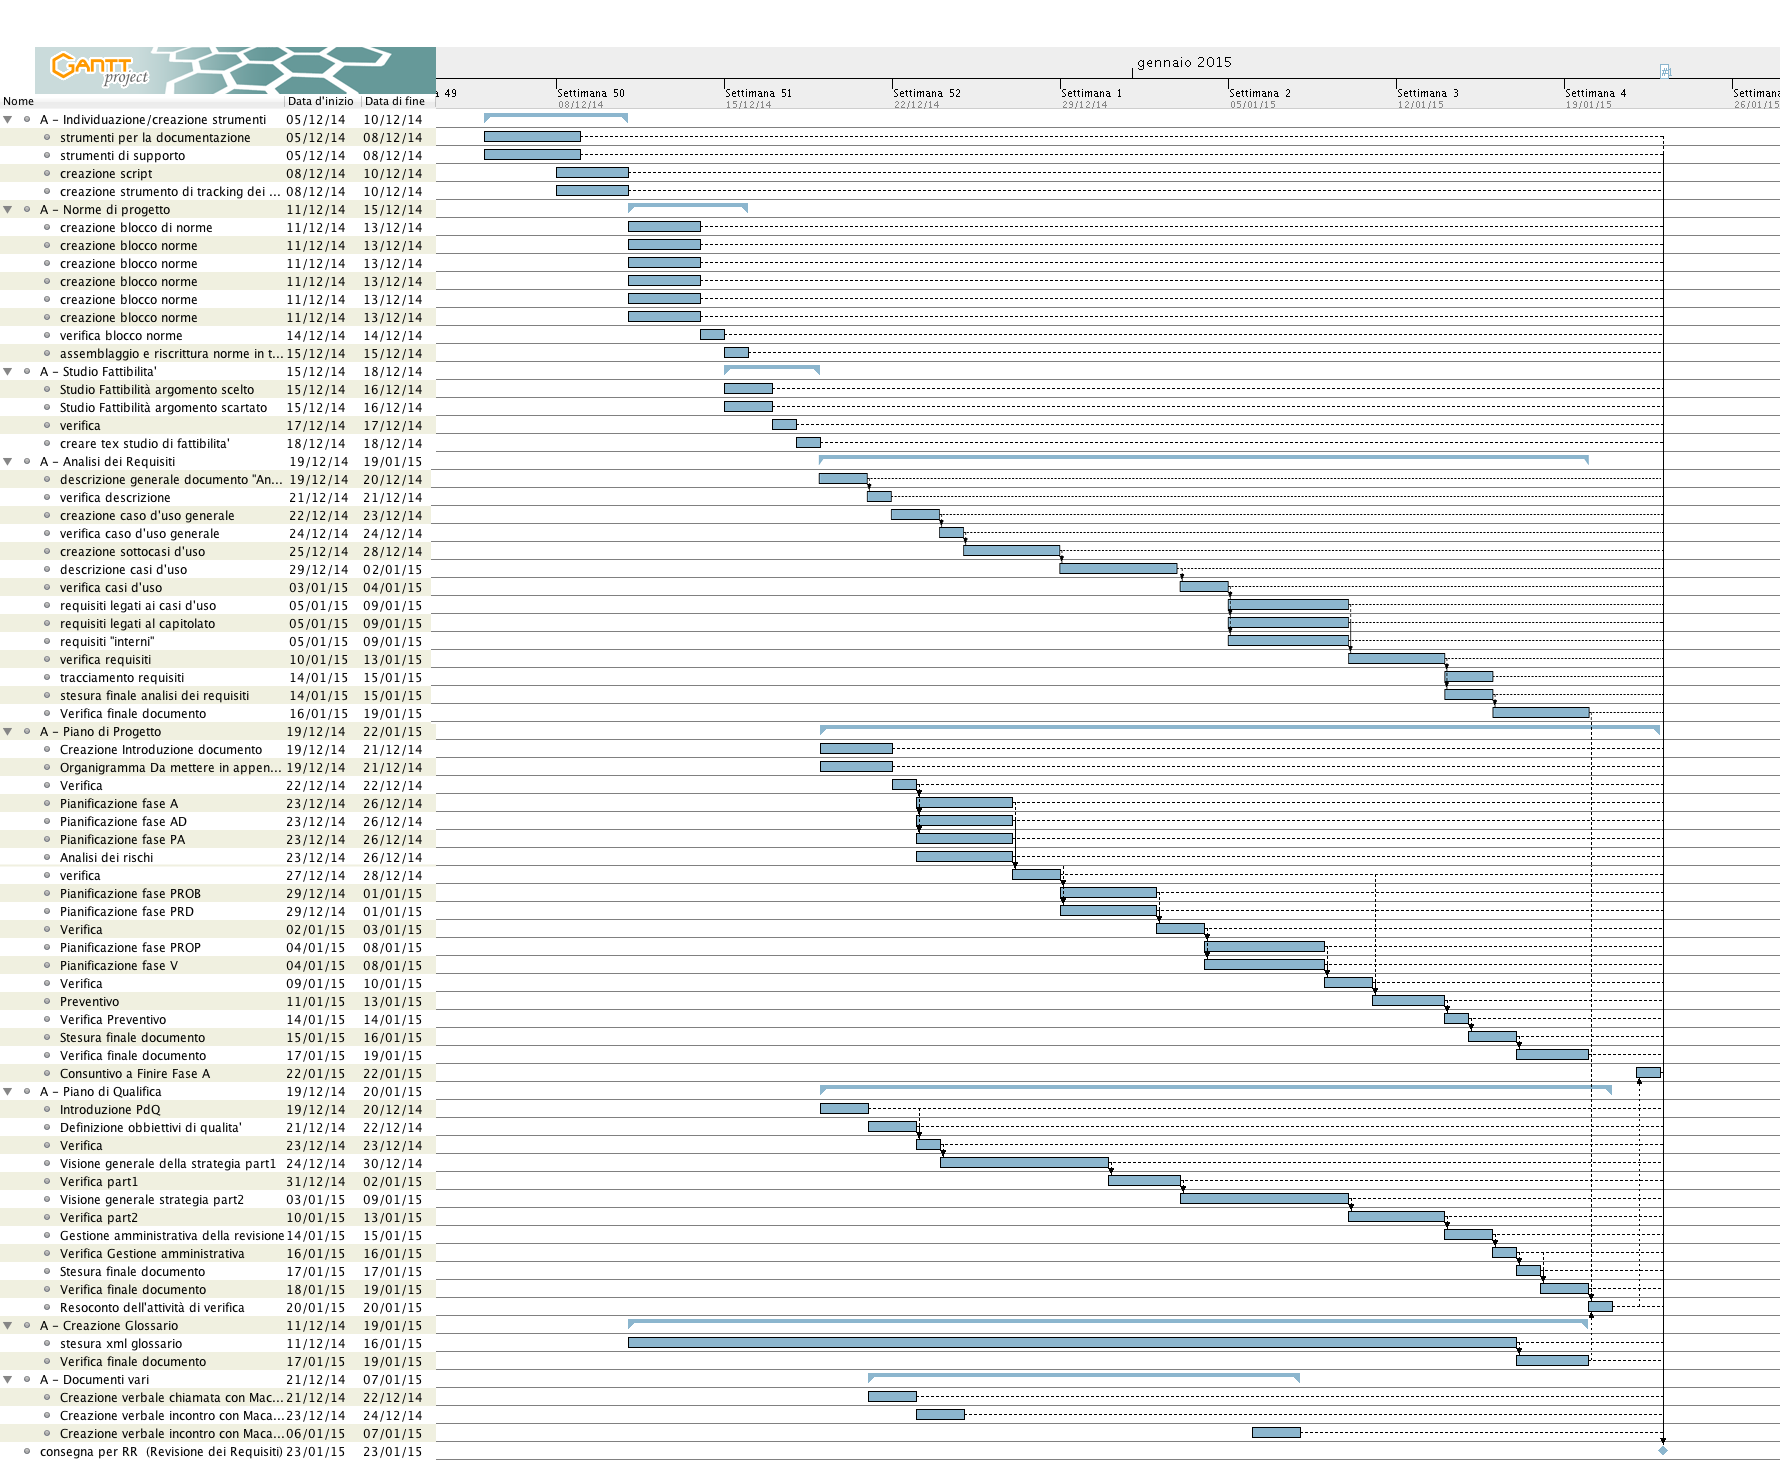
\includegraphics[width=\textwidth]{PianoDiProgetto/Pics/FaseDB.png}
	\caption{Gantt Fase DB}
\end{figure}
